\documentclass{esannV2}
\usepackage{amsmath,amssymb,graphicx,booktabs,microtype,lmodern,array}
\usepackage[T1]{fontenc}
\setlength{\textfloatsep}{10pt plus 2pt minus 2pt}\setlength{\floatsep}{8pt plus 2pt minus 2pt}

\title{Benchmarking Counterfactual Explanations\\of Model Change with Exact Ground Truth}
\author{Dinh Bao Bao, Tran Cong Minh and Le Hoai Bac
%
% DO NOT MODIFY THE FOLLOWING '\vspace' ARGUMENT
\vspace{.3cm}\\
%
% single institution: no "1- " numbering (ESANN template)
Faculty of Information Technology, University of Science \\
Vietnam National University, Ho Chi Minh City - Vietnam
}

\begin{document}
\maketitle

\begin{abstract}
Without ground truth one cannot tell which method for explaining a model update sees which change. We contribute a benchmark with exact ground truth and a linear analysis of what five families of explanations can see, among them differential counterfactuals ($\Delta$-CE): the nearest inputs on which exactly one model changes its decision by a margin. On gently fine-tuned null updates of small CNNs $\Delta$-CE finds no witness, also unfiltered and through a learned autoencoder (registered), while counterfactual and attribution differences report a change; cut to flag no null, counterfactual differences detect no offset. With two independent changes witnesses point to the one near the query (registered), as does the counterfactual of the new model checked against the old one, which, post hoc, misses the witnesses that carry the recovery of a shortcut. On small CNNs, not a ResNet-8, gradient differences are blind to an offset and see a rotation, as predicted; a registered hypothesis that $\Delta$-CE recovers the changed factor better than they do was rejected. Silence comes from the margin check, and a margin score tells whether decisions moved as well; what $\Delta$-CE adds is the search for witnesses a checked counterfactual misses.
\end{abstract}

\section{Introduction}

An update that improves accuracy can still change individual decisions in unwanted ways~\cite{yan}; explaining \emph{how} the models differ is a goal of explainable AI under distributional change~\cite{hammer,kaden}, distinct from explaining a shift of the data~\cite{kulinski}. Artelt et al.~\cite{artelt1,artelt2} compare the counterfactuals~\cite{wachter} of one input under each model, or a difference of gradients; Muschalik et al.~\cite{muschalik} compare feature importances; disagreement search~\cite{renard,deepxplore,digin} looks for inputs on which the models disagree. Ground-truth benchmarks exist for explaining one model~\cite{openxai,funnybirds,clevrxai}, not a change, so what each family can see goes unchecked.

We ask which kind of change each family can see, and add \emph{differential counterfactuals} ($\Delta$-CE): the closest input on the data manifold at which only $f_{new}$ changes its decision, both models by a margin $\kappa$; unlike robust counterfactuals~\cite{hamman,pawelczyk}, valid for both models, it seeks one valid for exactly one. It is a probe that should stay silent when nothing changed and otherwise return a checkable input.

\textbf{Contributions.} (i) A margin witness stays silent on gently fine-tuned null updates where counterfactual and attribution differences report change, also unfiltered and through a learned decoder; it localises two independent changes, and its search finds witnesses where a checked counterfactual of $f_{new}$ finds none. (ii) A benchmark with exact ground truth: five rendered factors, four shift types, null updates and a $4\times4$ grid over rotation and threshold. (iii) A linear analysis separating rotation from offset, tested on CNNs and a ResNet-8 under a protocol fixed in advance; all failures are reported.

\section{Differential counterfactuals and what each family sees}

Let $D:\mathcal Z\to\mathcal X$ map a search space onto the data manifold (here an exact renderer from factor space $\mathcal Z=[0,1]^5$). For class $y$ the margin is $m(z)=f_y(D(z))-f_{1-y}(D(z))$; $m_o,m_n$ belong to $f_{old},f_{new}$, and $h=m_n-m_o$. A query $z_0$ is valid if $m_o(z_0)\ge\kappa$ and $m_n(z_0)\ge\kappa$.

\textbf{Definition 1.} With $\mathcal F^N_\kappa=\{z: m_n(z)\le-\kappa,\ m_o(z)\ge\kappa\}$, a $\Delta$-CE of $z_0$ is $z^\star\in\arg\min_{z\in\mathcal F^N_\kappa}\|z-z_0\|$ if $\|z^\star-z_0\|\le r$, and NOT\_FOUND otherwise; swapping the models gives type O. Each $z\in\mathcal F^N_\kappa$ is a \emph{witness}: two forward passes verify that the models decide differently, both decisively, which a difference of two counterfactuals does not.

\textbf{Lemma 1.} Every witness has $h(z)\le-\kappa-m_o(z)\le-2\kappa$. Hence models whose margins differ by less than $2\kappa$ everywhere have no witness. \emph{Proof:} subtract the constraints of $\mathcal F^N_\kappa$.

\textbf{Corollary 1} (constant logit offset). If $f_{new}$ adds $b$ to the logit of class 1, e.g.\ the prior correction~\cite{saerens}, then $h\equiv\pm b$ and $\nabla h\equiv0$. Type-N witnesses exist only for the class whose margin $b$ lowers and only if $|b|\ge2\kappa$, at the points with $\kappa\le m_o\le|b|-\kappa$. \emph{Proof:} insert $h\equiv-|b|$ in Lemma 1; no linearity is needed.

\textbf{Linear case.} For linear margins on $\mathbb R^p$ write $\hat w_n=\cos\theta\,\hat w_o+\sin\theta\,v$ with $v\perp\hat w_o$, and let $d_n,d_o$ be the distances from $z_0$ to $\{m_n=-\kappa\}$ and $\{m_o=\kappa\}$. Gradient difference~\cite{artelt1}: $-(\hat w_n-\hat w_o)$; counterfactual differencing: $u_n-u_o$ (minimum-norm counterfactuals); witness: $u^\star$.

\textbf{Proposition 2.} (a) \emph{Offset} ($\theta=0$): the gradient difference is $0$; counterfactual differencing is a multiple of $\hat w_o$; a witness exists iff $d_n\le d_o$ and equals $-d_n\hat w_o$. (b) \emph{Rotation} ($0<\theta<\pi/2$): the gradient difference lies mainly along the new dependence $v$, the witness iff $\theta>\pi/4$ or $d_o(\sin\theta+\cos\theta)<d_n$; after projecting out $\hat w_o$ all three coincide up to scale, as in Theorem~1 of~\cite{artelt1} (new: the offset case and the witness). \emph{Proof} of (a): both normals equal $\hat w_o$; of (b): online supplement.

\section{Benchmark and protocol}

\textbf{Data and models.} Images are $32\times32$ ellipses rendered from five independent factors in $[0,1]$: aspect (task factor), size, colour, background and horizontal position; labels are $y=\mathbb 1[\text{aspect}>0.5]$ with 5\% noise. The exact renderer gives the factor change of any explanation without a learned oracle, and all methods search the same factor space through it. $f_{old}$ is a small CNN (five seeds); $f_{new}$ is $f_{old}$ fine-tuned on 10\,000 samples from one condition (Table~\ref{tab:changes}). A pair enters only if its change is visible in decisions on validation data. The ground truth is that of the injected change; what $f_{new}$ learns is measured by the realised rotation $\hat\alpha$ and threshold $\hat t$ of a logistic fit to its decisions (the grid is analysed at these).

\begin{table}[t]
\caption{Injected changes; $k^\star$: ground-truth factor. $^a$$\alpha\in\{0,.1,.25,.5\}\times t\in\{.5,.53,.56,.6\}$, 2 seeds; 4 offsets tested. $^b$Split D, 8 qualified; $^c$split G; both registered.}
\label{tab:changes}
\centering\footnotesize
\resizebox{\linewidth}{!}{%
\begin{tabular}{llllc}
\toprule
Change & Shift & Adaptation data & $k^\star$ & Pairs\\
\midrule
Shortcut & spurious & colour correlated with label (0.99) & colour & 3\\
Subgroup & local concept & labels flipped for size $>0.75$ & size & 3\\
Threshold & concept & $y=\mathbb 1[\text{aspect}>0.6]$ & aspect & 3\\
Null & none / covariate & resample / size $\sim U[0.5,1]$, same rule & --- & 5 / 3\\
Grid$^a$ & concept & $y=\mathbb 1[\text{aspect}+\alpha(\text{colour}-0.5)>t]$ & aspect / colour & 8 / 24\\
Offsets$^b$ & concept & grid, $\alpha=0$, $t\in\{.53,.56,.6\}$, seeds 2--4 & aspect & 9\\
Both$^c$ & spurious + local & Shortcut and Subgroup at once & colour, size & 8\\
\bottomrule
\end{tabular}}
\end{table}

\textbf{Metrics and methods.} Per pair: $N=300$ valid test points. $\mathrm{Recovery@}r$ is the share of points with a valid explanation within the budget whose largest factor change is $k^\star$ (NOT\_FOUND and ties count 0); it uses type-N witnesses only (pre-declared), so a query whose class the update raises counts 0. All counterfactual methods share one solver, the points and the budget $r=0.54$, set once on validation. We compare $\Delta$-CE ($\kappa=0.5$) with \textbf{CF-diff}, counterfactual differencing~\cite{artelt1}; \textbf{Grad-diff}, the gradient difference~\cite{artelt1}; \textbf{Imp-diff}, a difference of permutation importances~\cite{muschalik}, one vector per pair; \textbf{Seg-search}, a line search towards training points, after~\cite{renard}; \textbf{No-prox}, $\Delta$-CE without proximity, the DeepXplore objective~\cite{deepxplore}, to which DiG-IN~\cite{digin} corresponds on an exact manifold; \textbf{CF-new}, the counterfactual of $f_{new}$; and, in Section~4.3, IG-~\cite{ig} and SHAP-differences~\cite{shap}.

\textbf{Protocol.} Each test split served at most one confirmatory test, after all choices were fixed (splits A--G and their dates in the supplement); the follow-ups on splits D, F and G were registered before their data existed~\cite{osf}. Bootstrap intervals resample points within pairs, so Table~\ref{tab:tests} also counts pairs and the supplement repeats every test with the pair as unit. A digit tier and a label-shift update failed qualification.

\section{Results}

\begin{table}[t]
\caption{Recovery@$r$ (found-rate), split A, mean of 3 pairs (CIs $\pm0.035$); last row: found-rate, 8 nulls.}
\label{tab:results}
\centering\small
\resizebox{\linewidth}{!}{%
\begin{tabular}{lccccccc}
\toprule
 & $\Delta$-CE & CF-diff & Grad-diff & Imp-diff & Seg-search & No-prox & CF-new\\
\midrule
Shortcut & 0.38 (0.84) & 0.54 (0.93) & \textbf{0.91} (1.0) & 0.00 & 0.02 (0.08) & 0.35 (0.63) & 0.07 (0.93)\\
Subgroup & 0.53 (0.81) & 0.32 (0.99) & \textbf{0.62} (1.0) & 0.00 & 0.06 (0.10) & 0.29 (0.58) & 0.30 (1.0)\\
Threshold & 0.47 (0.47) & 0.76 (0.90) & 0.07 (1.0) & \textbf{1.00} & 0.07 (0.08) & 0.31 (0.40) & 0.90 (0.90)\\
Null & \textbf{0.000} & 0.994 & 1.0 & 1.0 & 0.000 & 0.000 & 0.996\\
\bottomrule
\end{tabular}}
\end{table}

\begin{table}[t]
\caption{Tests (95\% CIs; $^\dagger$90\%). Pairs: on the claimed side / all; $^\|$point level only ($\le4$ pairs, pair-level $p\ge0.0625$; other confirmed rows hold per pair). K: D = from a lemma or definition, R = risky prediction. When: pre/post = before any/after the first result (split B); grid = before the grid run; new = new data; reg = registered~\cite{osf}. Holm: $^{*}$, $^{\ddagger}$, $^{\S}$. $^\P$Run after its cost rule excluded it; expl.\ = exploratory; Proj.: $\hat w_o$ projected out.}
\label{tab:tests}
\centering\scriptsize
\setlength{\tabcolsep}{2.5pt}
\resizebox{\linewidth}{!}{%
\begin{tabular}{@{}llllcll@{}}
\toprule
Claim & Data & Estimate & $p$ & Pairs & Status & K, when\\
\midrule
\multicolumn{7}{@{}l}{\emph{Abstention and where}}\\
No witness on nulls & Null, B; Adult & 0/2\,400; 0/1\,500 & & 8/8; 5/5 & confirmed & D, post; new\\
No witness on unfiltered nulls & Null, D & 0/2\,400 & & 8/8 & confirmed & R, reg\\
Same, search via VAE decoder & Null, F & 0/800 & & 8/8 & confirmed & R, reg\\
No witness on nulls & ResNet-8, D$^\P$; E, $\kappa^\star$ & 180/200; 0/200 & & 0/2; 2/2 & not; expl. & R, reg; new\\
CF-diff (no cut) flags $|b|<2\kappa$ & Logit offsets & 0.961 [0.955, 0.967] & $2{\cdot}10^{-4}\,^{\S}$ & & confirmed & D, new\\
Witness $\ge$ margin score $+0.2$ & Offsets, D & $+0.17$ to $+0.97$ & & 7/8 & not conf. & R, reg\\
Witness localises ($L>0$) & Both, G & $L=0.50$ & 0.004 (sign) & 8/8 & confirmed & R, reg\\
\multicolumn{7}{@{}l}{\emph{Offsets}}\\
Grad-diff $<0.2$ & Grid, $\alpha=0$ & 0.081 [0.066, 0.096] & $4{\cdot}10^{-4}\,^{\ddagger}$ & 4/4 & confirmed$^\|$ & R, grid\\
Grad-diff $<0.2$ & Offsets, D & 0.033--0.093 & 0.004 (sign) & 8/8 & confirmed & R, reg\\
Grad-diff offset-free & Grid & $-0.098$ [$-0.143$, $-0.053$]$^\dagger$ & $0.94\,^{\ddagger}$ & & not conf. & R, grid\\
$\Delta$-CE $>$ Grad-diff & Threshold, B & $+0.31$ [0.27, 0.35] & $2{\cdot}10^{-4}\,^{*}$ & 3/3 & confirmed$^\|$ & D, post\\
\multicolumn{7}{@{}l}{\emph{Rotations}}\\
Grad-diff rises with $\alpha$ & Grid & $+0.57$ [0.53, 0.61] & $4{\cdot}10^{-4}\,^{\ddagger}$ & $\rho=0.89$ & confirmed & R, grid\\
Grad-diff $<0.2$; rot.\ $>$ offset & ResNet-8, D & 0.32--0.36; 0.06--0.10 & & 0/3; 0/3 & not conf. & R, reg\\
Proj.\ $\Delta$-CE $\approx$ Grad-diff & Shortc.\ B; grid & $-0.30$; $-0.35$ (CIs $\pm0.03$)$^\dagger$ & $1\,^{*}$; $1\,^{\ddagger}$ & & not conf. & R, post; grid\\
Normal at $z^\star$ halves gap or more & Grid, new & $-0.19\to+0.03$ [0.01, 0.05]$^\dagger$ & $6{\cdot}10^{-4}\,^{\S}$ & 4/4 & confirmed$^\|$ & R, new\\
\multicolumn{7}{@{}l}{\emph{$\Delta$-CE versus gradient differences}}\\
$\Delta$-CE $>$ Grad-diff & Subgroup & $-0.09$ [$-0.13$, $-0.05$] & & 0/3 & rejected & R, pre\\
Tie ($|\Delta|\le0.1$) & Shortc., Thresh. & $|\Delta|=0.17$--$0.53$ & & & not conf. & R, pre\\
\bottomrule
\end{tabular}}
\end{table}

\subsection{Abstention, detection and where}

\textbf{The witness stays silent when nothing changed.} On the 8 null pairs (Table~\ref{tab:results}), five null updates of an MLP on Adult, and 8 registered null pairs admitted without the original check, no query has a witness, while CF-diff attributes a change to 97.7--100\% of points (Table~\ref{tab:changes}: also covariate-shifted). Silence does not need the exact renderer: searching through the decoder of an autoencoder trained on the images (registered; run with 100 instead of 200 queries per pair, on CPU), no null query has a witness (0/800; CF-diff 85--94\%), while on 6 of 8 offsets witnesses exist for at least half of the lowered-class queries. The margin is what keeps the probe silent: with $\kappa=0$ witnesses appear on 83\% of null queries. The nulls are fine-tuned more gently than the offsets (3 epochs at learning rate $3{\cdot}10^{-4}$, not 10 at $10^{-3}$), though their threshold moves as much ($|\Delta\hat t|\le0.035$); the grid's null cell, fine-tuned like the offsets, has witnesses on 22\% of queries at $\kappa=0.5$, none at $\kappa=1$, where small grid offsets keep few (0.04).

\textbf{A margin score tells \emph{whether} as well.} With each score cut on the nulls to flag none, on the 8 registered offsets witnesses exist for 0.17--1.00 of the queries of the lowered class, the margin score flags 0.00--0.54 and CF-diff none. The witness beat the margin score by 0.2 in 7 of 8 pairs, not all as registered; no advantage for \emph{whether}.

\textbf{Witnesses show where.} In a registered update with a colour shortcut everywhere and a label flip for large objects, witnesses change size most for 46--75\% of queries near the large-object region and for 13--23\% far from it (difference $L>0$ in 8 of 8 pairs, pooled 0.50, sign test $p=0.004$). Grad-diff and CF-diff barely localise (0.09, 0.13), Imp-diff cannot; CF-new localises as well (0.51).

\textbf{Witness versus a checked counterfactual} (post hoc, saved outputs). The counterfactual of $f_{new}$ kept only where $m_o\ge\kappa$ is silent on the nulls too and localises ($L=0.48$), but finds witnesses for 0.42--0.46 of split-A queries against 0.47--0.84; $\Delta$-CE's extra witnesses carry its Recovery on Shortcut (0.38 vs.\ 0.03) and part on Subgroup (0.53 vs.\ 0.30), higher in 3 of 3 pairs each, not on Threshold (0.47 vs.\ 0.45). Minus the rate of naming $k^\star$ on nulls, $\Delta$-CE leads on Subgroup and Threshold (0.53, 0.47), Grad-diff on Shortcut (0.79); CF-new has $-0.09$ on Threshold.

\subsection{Offsets and rotations}

Gradient differences are blind to an offset, as Proposition 2(a) predicts: their Recovery is 0.081 on the pure offsets of the grid and 0.03--0.09 on the 8 registered offsets (8 of 8 below 0.2; sign test $p=0.004$). On Threshold (split B) $\Delta$-CE beats them (0.41 vs.\ 0.10) in 3 of 3 pairs, too few for a pair-level test. Type-N witnesses exist only on the side the offset lowers (Threshold: class 1), hence 0.47 in Table~\ref{tab:results}; type O covers the other side (nearer of N and O: 1.00, split C).

\begin{figure}[t]
\centering
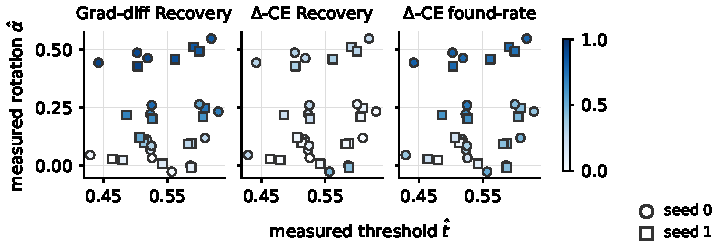
\includegraphics[width=0.85\linewidth]{figures/map_names.pdf}
\caption{Grid results at the measured rotation $\hat\alpha$ and threshold $\hat t$ of each $f_{new}$; colour scale 0--1; hollow: no $k^\star$; shape: seed of $f_{old}$.}
\label{fig:map}
\end{figure}

Gradient differences see a rotation, increasingly with its angle: Grad-diff Recovery rises from 0.36 at $\alpha=0.1$ to 0.93 at $\alpha=0.5$ ($t=0.5$) (Spearman $\rho=0.89$ over the 24 pairs, permutation $p=10^{-4}$; Fig.~\ref{fig:map}). The projection equivalence of Proposition 2(b) holds only with $\hat w_o$ taken at the witness (Table~\ref{tab:tests}).

\subsection{Attribution differences, other baselines, a second architecture}

With predictions logged beforehand, IG- and SHAP-differences recover colour on Shortcut (0.93) like Grad-diff and, against the predicted blindness, name aspect on Threshold (0.73--0.75 vs.\ 0.07), but also on 57\% and 71\% of null queries (IG-diff on 42\% of the registered nulls, as predicted): no signal. Imp-diff on test data ranks aspect first in all 9 change pairs, and $k^\star$ on adaptation data. Seg-search with ten times the segments finds witnesses for 0.26--0.47 of queries (predicted $\le0.2$), none that $\Delta$-CE misses.

On a registered ResNet-8, null fine-tuning moves margins four times more and witnesses appear on 0.90 of null queries: $\kappa$ is model-specific. With $\kappa$ calibrated on validation nulls (rule fixed in advance; grid extended after $\kappa\le2$ failed), $\kappa^\star=2.5$, no new null query has a witness (0/200) and witnesses exist for 0.78--1.00 of lowered-class offset queries ($\Delta$-CE Recovery 0.36--0.40). Grad-diff sees neither change: on split D (2 null, 3 offset, 4 rotation pairs) it names aspect on 0.32--0.36 of offset queries, near its 0.20--0.30 on nulls, and on rotations its Recovery, 0.06--0.10, is below the offset of equal seed and threshold in the 3 comparable pairs.

\section{Discussion and limitations}

Silence comes from the check $m_o\ge\kappa$, which a counterfactual of $f_{new}$ can be given; specific to $\Delta$-CE is the search for witnesses where that counterfactual is not one. \textbf{Limitations.} (1) The data are synthetic and binary; Recovery through the learned decoder is approximate and lower for $\Delta$-CE than for CF-diff; multi-class tasks, other domains, retraining from scratch and architecture changes are untested; the tabular test covers abstention only. (2) $\kappa$ is in logit units, exact only for a constant offset, and must be calibrated on null updates of each model family and fine-tuning recipe. (3) Witnesses see only decisive changes on the manifold within the budget, without a certificate. (4) Several tests were formed after earlier results; changes were logged before their data existed, with three disclosed exceptions; online supplement and code: github.com/Johnlrr/explaining-model-change.

\begin{footnotesize}
\begin{thebibliography}{20}
\setlength{\itemsep}{0pt}\setlength{\parskip}{0pt}
\bibitem{yan} S. Yan et al. Positive-congruent training: towards regression-free model updates. \emph{CVPR}, 2021.
\bibitem{hammer} B. Hammer, E. H\"ullermeier. Interpretable machine learning: on the problem of explaining model change. \emph{Workshop Comput.\ Intell.}, 2021.
\bibitem{kaden} M. Kaden et al. Reliable counterfactuals for machine learning models -- current aspects and perspectives. \emph{ESANN}, 2026.
\bibitem{kulinski} S. Kulinski, D. I. Inouye. Towards explaining distribution shifts. \emph{ICML}, 2023.
\bibitem{artelt1} A. Artelt et al. Contrastive explanations for explaining model adaptations. arXiv, 2021.
\bibitem{artelt2} A. Artelt et al. Contrasting explanations for understanding and regularizing model adaptations. \emph{Neural Process.\ Lett.}, 2022.
\bibitem{wachter} S. Wachter et al. Counterfactual explanations without opening the black box. \emph{Harv.\ JOLT}, 2017.
\bibitem{muschalik} M. Muschalik et al. Agnostic explanation of model change based on feature importance. \emph{KI}, 2022.
\bibitem{renard} X. Renard et al. Understanding prediction discrepancies in machine learning classifiers. arXiv, 2021.
\bibitem{deepxplore} K. Pei et al. DeepXplore: automated whitebox testing of deep learning systems. \emph{SOSP}, 2017.
\bibitem{digin} M. Augustin et al. DiG-IN: diffusion guidance for investigating networks. \emph{CVPR}, 2024.
\bibitem{openxai} C. Agarwal et al. OpenXAI: towards a transparent evaluation of model explanations. \emph{NeurIPS}, 2022.
\bibitem{funnybirds} R. Hesse et al. \mbox{FunnyBirds}: a synthetic vision dataset for a part-based analysis of explainable AI methods. \emph{ICCV}, 2023.
\bibitem{clevrxai} L. Arras et al. CLEVR-XAI: a benchmark dataset for the ground truth evaluation of neural network explanations. \emph{Inf.\ Fusion}, 2022.
\bibitem{hamman} F. Hamman et al. Robust counterfactual explanations for neural networks with probabilistic guarantees. \emph{ICML}, 2023.
\bibitem{pawelczyk} M. Pawelczyk et al. On counterfactual explanations under predictive multiplicity. \emph{UAI}, 2020.
\bibitem{saerens} M. Saerens et al. Adjusting the outputs of a classifier to new a priori probabilities: a simple procedure. \emph{Neural Comput.}, 2002.
\bibitem{ig} M. Sundararajan et al. Axiomatic attribution for deep networks. \emph{ICML}, 2017.
\bibitem{shap} S. Lundberg, S. Lee. A unified approach to interpreting model predictions. \emph{NeurIPS}, 2017.
\bibitem{osf} Registrations of the follow-up experiments. OSF, 2026. osf.io/vfjtk, osf.io/fr7jv, osf.io/fp8uc
\end{thebibliography}
\end{footnotesize}

\end{document}
